\part{Application}
\chapter{Inertial Waves in a Rotating Cone}

\section{Introduction}

Following the introduction and validation of the immersed boundary methods for No-Slip boundaries,
we now want to exemplarly investigate a fluid system using these methods
and find out if we can reproduce some of the expected physical properties.\\
In relation to the research focus of the geophysical fluid mechanics research group, there are a variety
topics of interest.
One area of research lies in the exploration of dynamo effects in geological and stellar system.
In particular this means the generation of magnetic fields by electrically conducting fluids on large scales.
In this thesis we will not consider MHD-equations.
However in general it is considered that the helicity of a fluid domain $\Omega$, given by
\begin{align}
    \int_{\Omega}\dif V  \vec{u} \left( \nabla \times \vec{u} \right)
\end{align}
is directly linked to dynamo action [CITE].
Therefore, beside inertial wave propagation we want to observe a possible large helicity.
For the system we describe in the following section one further application
would be to study inertial wave excitaton by turbulence. (MORE DETAIL THIS AND ALPHA FUNCTION)

\section{Theoretical Description}

The objective we have in mind is the numerical computation of inertial wave excitation inside a liberating cone.
A theoretical discussion of this system  can by found in \citep{GREENSPAN}.
Here we want to orient towards an experiment which was being performed by \citep{Beardsley1970}

The schematic setup of the experiment is shown in figure ().
It contains of a cone given by the radius $R$ and the height $h$, resulting into an angle $\alpha = \tan()$.
The cone is rotating with a modulated frequency

\begin{figure}[!bp]
  \begin{minipage}[c]{0.6\textwidth}
      \centering
        \resizebox{0.7\textwidth}{!}{
       \import{gfx/cone//}{cone.pdf_tex}
      }
  \end{minipage}
  \begin{minipage}[c]{0.3\textwidth}
      \caption{Numerical setup of the cone, oriented on the experiment. The total heigth is given by $h$, whereas the height of the cone is set to $h_c$.
      The winkel alpha defines the slope and $h_t$ the cutoff from the bottom.}
      \label{cone:theorie}
  \end{minipage}
\end{figure}


\begin{align}
\Omega(t) = \Omega_0 + \epsilon \omega \cos(\omega t)
\end{align}

The modulation of the rotation frequency is also denoted as libration [RIGHT?] and can be used as a possible mechanism
for inertial wave exitation [CITE].
The overall idea of the setup is to introduce a geometry containing a singularity and study the influence on the ability of
the system to develop inertial eigenmodes.
Let us recall that the dispersion relation and group velocity of an inertial wave paket is given by

\begin{align}
    \omega = \frac{2\vec{\Omega}\vec{K}}{K} = 2 \Omega \cos\Theta ; \vec{c}_g = -\frac{2\vec{K}\times (\vec{\Omega} \times \vec{K})}{K^3}
\end{align}

with the wavenumber $\vec{K}$.
Let us now consider the propagation of an interial wave paket from the top edge of the cone as shown.
As discussed in section (), the reflection of inertial waves up on a  plane wall is a violation of snell's law.
For each reflection the propagation angle with respect to the rotation axis stays constant,
whereas the group velocity decreases.
It can be shown that for all path i.e. $L$ and $L^o$ the propagation time of the wave energy stays constant [CITE]
\begin{align}
    \frac{K^o}{K} = \frac{\cos(\Theta - \alpha)}{\cos(\Theta + \alpha)}
\end{align}
This means that the overall propagation time into the apex of the cone becomes infinity, along with the energy density and the wave number.
In conclusion it follows that since no reflection out of the cone apex can occur, the possibilty of inertial eigenmodes is not given.\\
In the experimental setup described by [] the experiment was compared to another setup where the cone was replaced with a frustum of a cone,
thus a bottom blade to enable the reflection of inertial waves was inserted.
As a result for the cone, a continuos wave spectrum could be observed in comparision to a discrete spectrum  for the frustum.\\

\newpage

\section{Numerical Implementation of Liberation}

For the numerical implementation of the experiment, we will use a modified set of the equations
introduced in section \ref{THEORE:ROT}.
We have to concern that the system has now a time-depent rotation rate.
For the non-dimensional system, with $\vec{u}^* =  \vec{u} (|\vec{\Omega}|L)^{-1}$, we set

\begin{align}
    \vec{\Omega(t)} = 1 \; + \; \epsilon \cos(\omega t)\vec{e}_z
\end{align}

There are two options, which should be considered here.
First of all, we can choose a rotating coordinate system with a constant velocity $\Omega_0$.
This means the we can directly use the equations () to (), however since the overall rotation rate of the system is
modulated, it is necessary to introduce the boundary conditions

\begin{align}
    \vec{v}|_{Border}  = \Omega \times \vec{r} = \begin{bmatrix}
           -y \epsilon \cos(\omega t) \\
           -x \epsilon \cos(\omega t) \\
           0\\
         \end{bmatrix}
\end{align}

The alternative option is the introduction of a accelerated frame of reference.
In this case the boundary conditions do not need to be modified, but the coriolis forcing term is given by (CITE)

\begin{align}
    \vec{f} &= 2 \vec{\Omega} \times \vec{v} + \pdn[]{t}\left(\vec{\Omega} \times \vec{v} \right) \\
            &= \begin{bmatrix}\\
           -y \epsilon \cos(\omega t) \\
           -x \epsilon \cos(\omega t) \\
           0\\
         \end{bmatrix}
            &= \begin{bmatrix}\\
           -y \epsilon \cos(\omega t) \\
           -x \epsilon \cos(\omega t) \\
           0\\
         \end{bmatrix}
\end{align}

In the last step a linearization of the equation was performed.
Since we are in interested in the propagation of intertial modes this
step was performed to eleminate all possible non-linear effects which could occur.
Furthermore the non-linear advection term was removed from the equations.

-stability contstraints
-default

-additional constraint time for wave to trave along cylinder smaller than bla \citep{TILGNER, OGOEPFERT}.
\begin{align}
    t_{c} = \sqrt{\frac{2}{c^2}} << 2\pi
\end{align}
-result $c^2 = 500$ in absprache mit ogoepfer und tilgner.



\newpage

\subsection{Setup}

We will now introduce the numerical setup which has been used for the simulations carried



\begin{figure}[!bp]
  \begin{minipage}[c]{0.6\textwidth}
      \centering
        \resizebox{0.7\textwidth}{!}{
       \import{gfx/cone/conesim//}{setup.pdf_tex}
      }
  \end{minipage}
  \begin{minipage}[c]{0.3\textwidth}
      \caption{Numerical setup of the cone, oriented on the experiment. The total heigth is given by $h$, whereas the height of the cone is set to $h_c$.
      The winkel alpha defines the slope and $h_t$ the cutoff from the bottom.}
      \label{cone:setxp_image}
  \end{minipage}
\end{figure}

\clearpage

\section{Simulation of a Liberating Cylinder}
\label{cone:sec:lib_cylinder}


As a first step towards the implemenation of the cone,
we want to simulate fluid flow in a liberating cylinder.
The reason for this is, that we initially want to
compare the results of different immersed boundary methods to each other,
before choosing one method for the liberating cone.
Furthermore the system has already been rigorously studied, such that
we can make a comparison to the available theoretical and numerical results.\\

-theoretically greenspan  blabla

The velocity of a mode is given by in cylindr. coord

\begin{align}
    u_r =  1
\end{align}


-mode kann dann festgelegt werden durch tuple bla.\\
The numerical setup is  given by ..
-Nx  = 128 ,lx, ly
-aspect ration
-ekman number
-further condition timestep
-omega in bla
\newpage

\subsection{Results \& Discussion}




\begin{align}
    \left<v_z^2 \right>(t) =  \int \dif V v_z(t)^2 \approx \sum_{i, j, k}^{N_x,N_y,N_z} \Delta x \Delta y \Delta z \left.v_z(t)^2 \right|_{i,j,k}
\end{align}

\begin{align}
    A\left(\left<v_z^2\right>\right) = \frac{\max(\argmax(\left<v_z^2\right>_{v})) - \max(\argmin(\left<v_z^2\right>_{v}))}{2}
\end{align}

-bilder
-description


\begin{figure}[!pt]
  \centering
  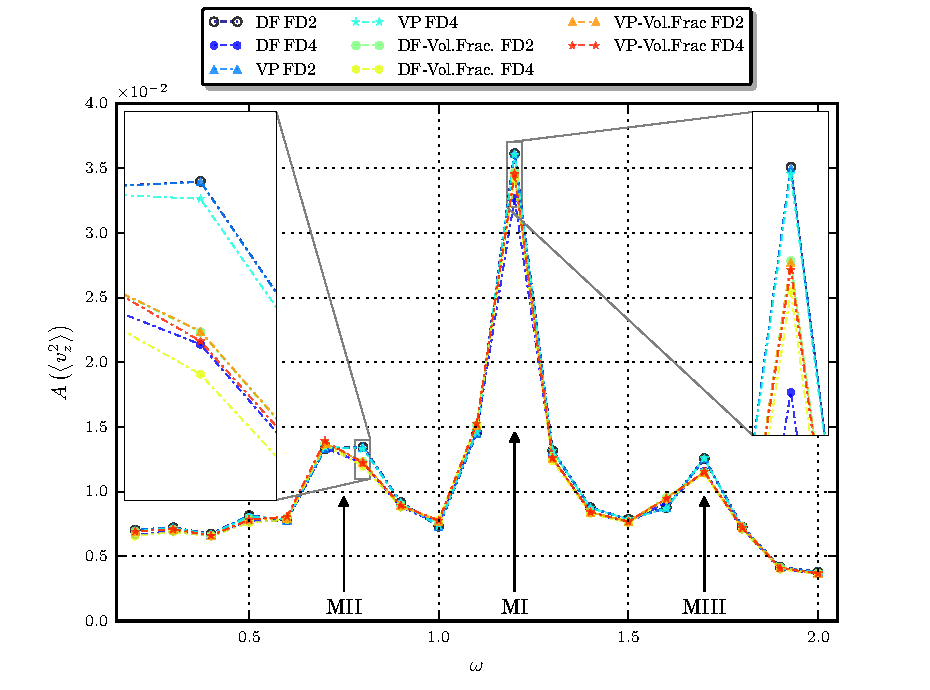
\includegraphics{gfx/cone/cylinder/cylinder.pdf}\label{fig:cone:cyl}
  \caption{blabla}

  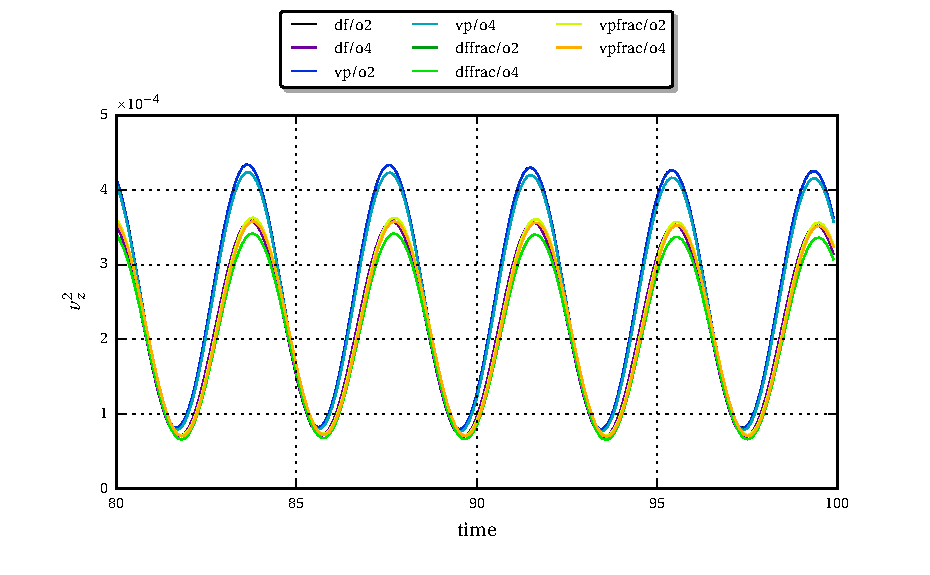
\includegraphics{gfx/cone/cylinder/cyl_vz.pdf}\label{fig:cone:cyl_time}
  \caption{blabla}
\end{figure}
\newpage

-behaviour known theorie
- paper kurz erklären symetrie warum fehlen bestimmte moden ? ?

As a first system we want to investigate the

- erstes test system cylinnder\\
- expectation

- verglein von den bedien implementierungen\\
- first test omega = 1.2 ...\\
- diskussion rand compare to tcflow \\
- test serie verschiede methoden\\
- spektrum dargesstel\\
- evtl raytracer  comparison
- heliziätte dargstellt\\
- results diskussion ip kaputt heli 0 etc \\
\subsection{Numerical Viscosity}

\newpage

\section{Simulation of a Liberating Cone}

In this section we will discuss the different numerical simulations, which has been performed
with a liberating cone. We begin with the comparison to the experiment performed by \citep{Beardsley1970}.
As a next step we analyse the physical behaviour when performing the transition from a cylinder
to a cone and finally  we will investigate the influence of different offsets on top of the cone.
All simulations performed in this section use the introduced setup with different geometric parameters.
As a IBM we choose the direct forcing  method of second order.

-as a convention we refer to frustom cone etc

\subsection{Simulation of the Experiment}

The setup for this simulation is oriented on the experimental setup given by \citep{Beardsley1970}, which
we disussed in section ().
In the first part of the experiment a plexiglass cylinder of height $H=\SI{19.95}{\centi\meter}$ and a radius of
$r=\SI{19.95}{\centi\meter}$ was used. The apex half angle was set to $24^{\circ}3.7^{\prime}$ degree,
which relates to our setup with $\alpha=65^{\circ}56.3^{\prime}$
For the rotation rate a frequency of $\omega =\SI{6.28}{\radian\per\second}$ was chosen.
As a fluid, water was used, the resulting viscosity,given by \citep{tipler2003}, is $\nu = \SI{1.0}{\milli\pascal\second}$.
The resulting Ekman number is given by

\begin{align}
    \Ekman = \frac{\nu}{\omega r H^2} \approx 7.72\cdot 10^{-6}
\end{align}

In the second part of the experiment the apex of the cone was replaced by a frustum through the
insertion of a bottom plate at the position $z/H = 0.261$.
For the simulation we choose an Ekman number of $\Ekman =  10^{-4}$, since a simulation of higher ekman numbers is
diffcult to realise due to the computational effort.
Furthermore we set $\alpha = \arccos(1/2) = 60^{\circ}$, $H=1$ and $r=0.5$.\\
This means that for $\omega=1$, the propagation of an inertial wave package is parallel to the slope of the cone.
For the offset on top of the cone, we obtain the condition

\begin{align}
    o = H - h_c =  1 - r\tan{\alpha} \approx 0.134
\end{align}

The simulation has two setups in analogy to the experiment.For the second part the bottom plate is set to $h_b=0.25$.
A series of simulations of these systems where performed, with the parameters

\begin{center}
\vspace*{0.7ex}
\begin{tabular}{c|c|c|c|c|c|c }
%\begin{tabular}{p{0.1\linewidth}| p{0.1\linewidth}| p{0.1\linewidth}|  p{0.1\linewidth}| p{0.1\linewidth}| p{0.1\linewidth} }
$ \leftarrow  \omega \rightarrow $ & $\Delta t$ & $\Delta x$ & $c^2$ & \Ekman  & $l_x, l_y, l_z$ & $T_{end}$\\
\hline
$[0.2,\; 2], \Delta w = \nicefrac{1}{10}$ & $10^{-5}$ & $\nicefrac{1}{128}$ & 500 & $10^{-4}$  & (\{1, 0.75\}, 1, 1) & 100\\
\end{tabular}
\vspace*{0.7ex}
\end{center}

\clearpage
%\begin{figure}[!tp]
%  \begin{minipage}[c]{0.6\textwidth}
%      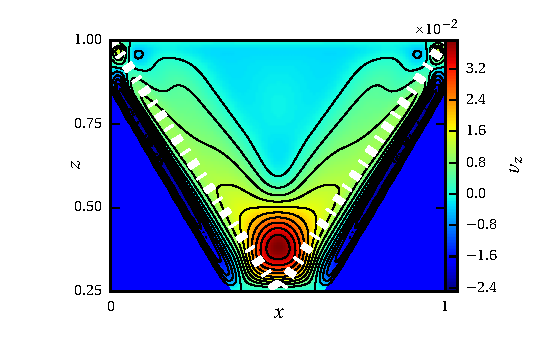
\includegraphics{gfx/cone/experiment/contour.pdf}\label{fig:mask_vp}
%  \end{minipage}\hfill
%  \begin{minipage}[c]{0.3\textwidth}
%  \caption{Stability regions for $\Omega_s$ for different Runge-Kutta methodsi
%    Stability regions for $\Omega_s$ for different Runge-Kutta methodsi
%  }
%  \label{fig:num_rkstab}
%  \end{minipage}
%\end{figure}
%
%\begin{figure}[!tp]
%  \begin{minipage}[c]{0.3\textwidth}
%  \caption{Stability regions for $\Omega_s$ for different Runge-Kutta methods
%  Stability regions for $\Omega_s$ for different Runge-Kutta methodsi
%  }
%  \label{fig:num_rkstab}
%  \end{minipage}
%  \hfill
%  \begin{minipage}[c]{0.6\textwidth}
%      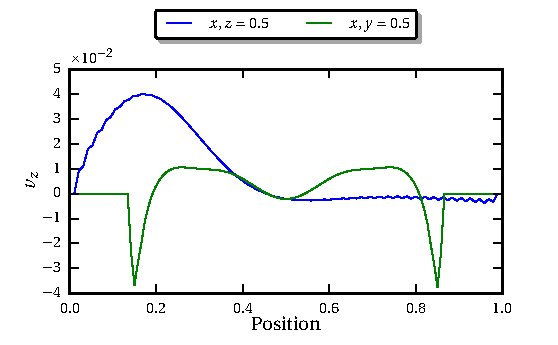
\includegraphics{gfx/cone/experiment/error.pdf}\label{fig:mask_vp}
%  \end{minipage}
%\end{figure}

\begin{figure}[!bp]
  \centering
  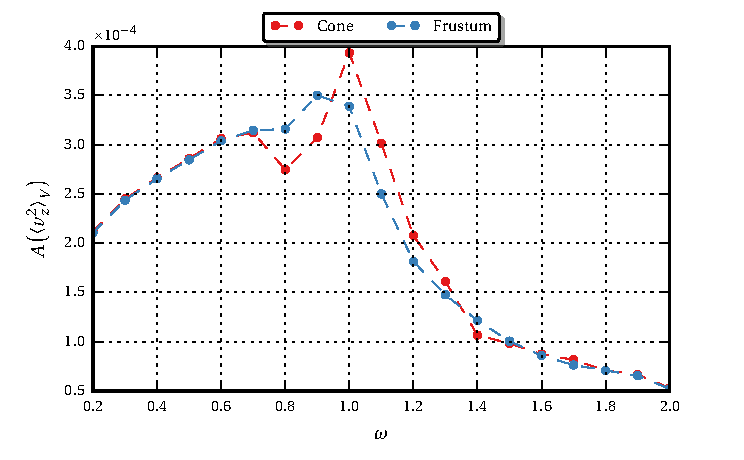
\includegraphics{gfx/cone/experiment/experiment.pdf}
  \caption{Amplitude $A\left(\left<v^2_z\right>_V\right)$ as a function of the liberation frequency $\omega$,
            for a cone and a frustum.  \label{fig:cone_expseries} }
\end{figure}

\subsubsection{Results \& Discussion}
\label{cone:exp}

The results of the simulations are shown in figure \ref{fig:cone_expseries}.
For both cases, the frustum and the cone, we can observe an increase in $A\left(\left<v^2_z\right>_V\right)$
from $\approx 2\cdot10^{-4}$ at $\omega=0$ to  $\approx 3.4\cdot10^{-4}$ for the frustum and $\approx 4\cdot10^{-4}$ for the cone,  at $\omega=1$.
From here one the Amplitude decreases to $\approx 5\cdot10^{-5}$ at $\omega=2$.\\
A difference between the two setups can be observed in the surrounding area of $\omega=1$.
For the cone the increase of the amplitude is interrupted at $\omega=0.6$, a minimum can be observed at $\omega=0.8$, followed by
a peak at $\omega=1$. For the frustum the minium is not directly visible but it can be noted that the
amplitude does not increase as much at $\omega=0.7$, as for lower frequencies.\\
The maximum occurs at $\omega=0.9$, in comparison to the cone we see an increase in the amplitude of $\approx 5\cdot10^{-5}$.
However, it has to be considered, that due do the stepwidth of $\Delta \omega = 0.1$, the exact position of the maxima is
not apparent.\\
One possible assumption, regarding the position of the maximum with respect to the frequency, is that
the expansion of the frustum with a tip  results in a shift to lower frequencies.
The left shift in the decrease for $\omega > 1$ furthermore supports this idea.\\
Overall it appears that the spectrum can be divided into two domains $\Omega_1~=~\{0\leq\omega<1$\} and $\Omega_2~=~\{1\leq\omega\leq2\}$.
This result is not unexpected, since we choose the slope $\alpha$ of the cone such that for $\omega=1$, it is parallel
do the group velocity $\vec{c}_{g}$.
For $\omega\in\Omega_1$ the results for both setups are similar, since in this domain, the cone tip does not act as an attractor.
An inertial wave propagates the top, after a reflection on the side of the cone.
Hence, for both setups we obtain a similar spectrum.
The differences occur when $\omega$ is reaching the critical slope, in this scenario an inertial wave propating from the
top edges, travereses directly into the apex of the cone, or is reflected slightly at he bottom plate of the frustum.
As a results we see the increase in the amplitude.
For $\omega\in \Omega_2$ we would expect further reflections for the frustum, however the similar
decay of the amplitude refutes this assumption.\\
The results of the simulation do not match with the ones of the experiment we discussed in section ().
A possible explanation we want to propose here, is the use of a different Ekman number, which is of order $10^{-4}$ in contrast
to the one of the experiment of $10^{-5}$.
As a consequence the width of an inertial wave packet, given by $\propto \Ekman^{1/3} \approx 2\cdot10^{-2}$ (see \citep{} or section...),
is around twice the size as in the experiment. We assume that as a results a wave reflecting on the bottom of the frustum
is strongly damped due to wall friction.
DISCUSS T:\\
damping  could be propt $\Ekman \vec{K}$.

\subsection{Transition to from a Cylinder to a Cone}

We now want to further investigate the results from the previous simulation.
The assumption was made, that the inserted bottom plate is to narrow to support an efficient reflection
of inertial waves, due to frictional losses at the bottom of the cone. Thus, the next objective would be to
test the influence of different gap radii $r$.\\
We propose a setting where we begin with the possible largest bottom gap, which is $r=0.5$.
As a next step we iteratively decrease the size of the gap by $\Delta r = 0.125$ until $r=0$ is reached.
An alternative approach to this woudld be to change the offset from the bottom of the cone, which would result in a constant
slope but different heights of the simulation domain.
The influence on the simulation domain is shown in figure ()(b).
For $r=0.5$ the domain is given by a cylinder, which than transforms into a cone with a frustum and finally with an apex for $r=0$.
The simulation parameters are given by

\begin{center}
\vspace*{0.7ex}
\begin{tabular}{c|c|c|c|c|c|c|c }
%\begin{tabular}{p{0.1\linewidth}| p{0.1\linewidth}| p{0.1\linewidth}|  p{0.1\linewidth}| p{0.1\linewidth}| p{0.1\linewidth} }
$\leftarrow r \rightarrow$ & $ \leftarrow  \omega \rightarrow $ & $\Delta t$ & $\Delta x$ & $c^2$ & \Ekman  & $l_x, l_y, l_z$ & $T_{end}$\\
\hline
$[0,\; 0.5], \Delta r =0.125$ & $[0.2,\; 2], \Delta w = \nicefrac{1}{10}$ & $10^{-5}$ & $\nicefrac{1}{128}$ & 500 & $10^{-4}$  & (1, 1, 1) & 100\\
\end{tabular}
\vspace*{0.7ex}
\end{center}
%
%\subsubsection{Results \& Discussion}
%\begin{figure}[!bp]
%      \begin{minipage}[c]{0.4\textwidth}
%      \centering
%        \resizebox{0.8\textwidth}{!}{
%       \import{gfx/cone/transition//}{attractor.pdf_tex}
%      }
%      \end{minipage}\hfill
%  \begin{minipage}[c]{0.6\textwidth}
%      \caption{
%          Wave attractor in a cylinder $\left(\text{\colorbox{green}{\textcolor{green}{o}}{\null}}\right)$
%          and shifted\\ attractor $\left(\text{\colorbox{red}{\textcolor{red}{o}}{\null}}\right)$
%          for $r<0.5$. To maintain the same attractor the point of reflection has to be at the same height $h_r$.
%      }
%      \label{cone:theorie}
%      \end{minipage}\hfill
%\end{figure}



\subsubsection{Results \& Discussion}

The results of the simulations are shown in figure \ref{fig:cone:transition}.
For $r=0$ we can see the inertial modes of a liberating cylinder, which is in accordance
to the results we discussed in section \ref{cone:sec:lib_cylinder}.
With an decrease of the radius we can observe a change in the position and amplitude of the
inertial modes. We want to exemplarly discuss this pattern for the (2, 2) mode at $\omega=1.3$, where it is the best visible.
For all other modes the transition results in a similar behvavior.\\

\begin{figure}[!pt]
  \centering
  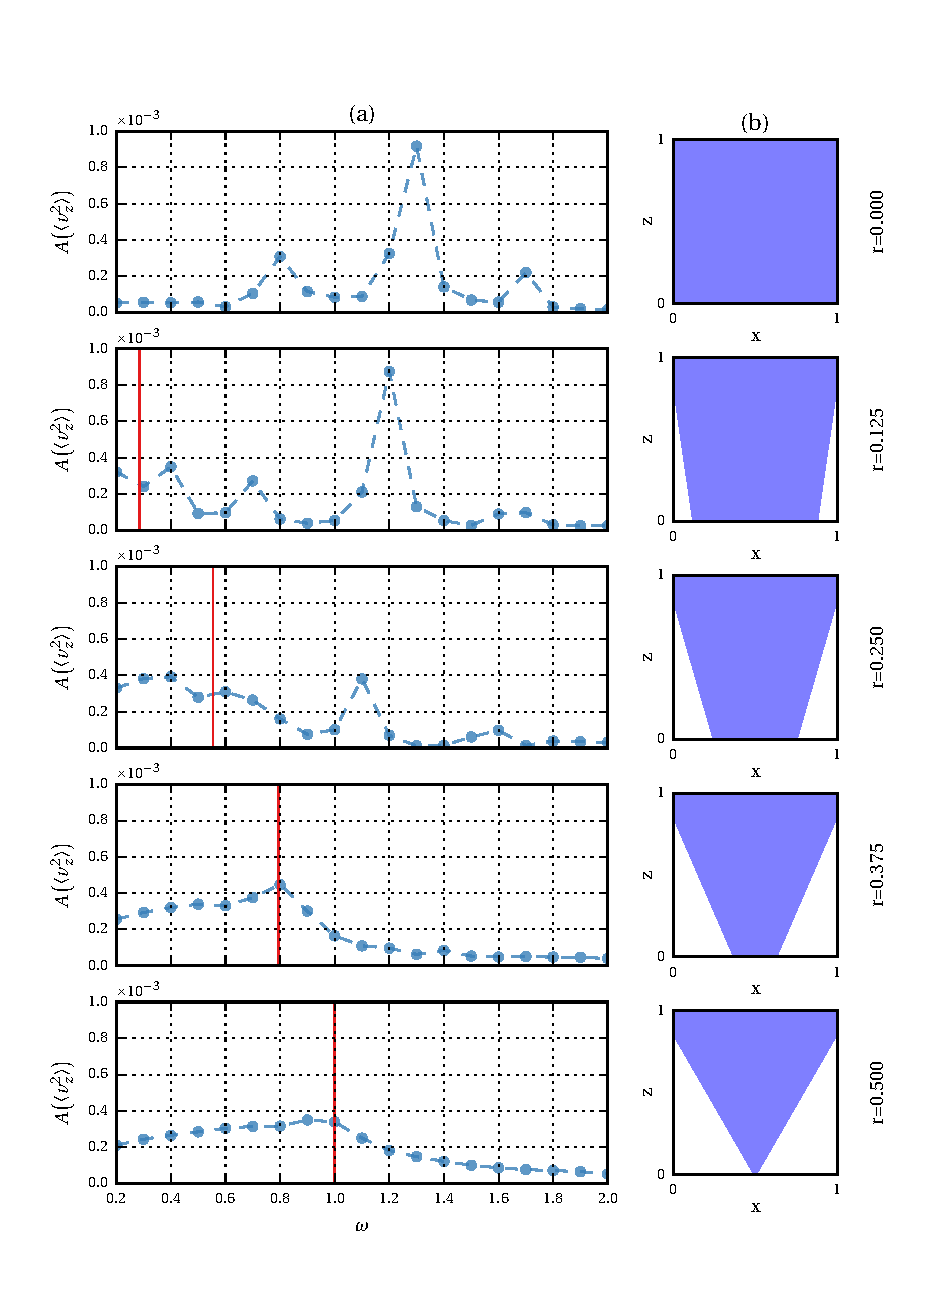
\includegraphics{gfx/cone/transition/transition.pdf}
  \caption{\label{fig:cone:transition}
    Simulation of
  }
\end{figure}

The decrease of the radius leads to a shift to lower frequencies of the (2, 2) mode,
from $r=0$ to $r=0.375$ it is of the order $\Delta \omega=0.1$.
Furthermore we can see, that during the transition a damping of the mode occurs.
For $r=0.5$ the amplitude is of order $\approx8.9\cdot10^{-3}$, for $r=0.375$ it is
$\approx8.9\cdot10^{-3}$ and for $r=0.25$ we obtain $\approx3.8\cdot10^{-3}$.\\
Whereas the first decrease of the radius does not significantly affect the amplitude,
the second decrease leads to a strong damping to less than half of the original size.
With a further decrease in $r$, the (2, 2) mode is annihilated.
\footnote{ for the possible (1, 2) mode we still can observe a slight increase of the amplitude at $r=1.4$}
One possible explanation for the shift can be given
by having a look at the inertial mode structure, for different radii as shown in figure \ref{fig:cone:phase}.\\
For $r=0.5$ we have an inertial mode, which is symmetric to the plane $h/2$.
In this plane, the waves excited from the bottom and top of the cylinder, annihilate each other and form a wave node.
An decrease of radius breaks the axial symetrie of the inertial mode.
As a result only a distorted version of the mode can exist, where the center of the wave node
is given by the intersection of the diagonals from the top to the bottom edges of the frustum.
In order to obtain the new shape it is necessary to increase the propagation angle $\Theta$,
which is equivalent to lowering the liberation frequency.
We can furthermore say that for $r \rightarrow 0$, the center given by

\begin{align}
c  = r \frac{h}{r+\nicefrac{l_x}{2}}
\end{align}

converges against zero, hence a mode cannot exist in this state.
Beside the changes of the inertial modes it can be noted, that simultaneously to the decrease of the radius,
a lift of the amplitudes at lower frequencies occurs.
The vertical lines in figure \ref{fig:cone:transition} are set to the position $\omega=\Theta$.
The area $\omega<\Theta$ can again be associated with the frequency domain, where the wave propagation angle $\Theta$ is larger than
the  slope of the cone $\alpha$ and waves propgate to the top, up on reflection on the slope.
For $r=0$ we have the indentical setup to the simulation in section \ref{cone:exp}.

\begin{figure}[!pt]
  \centering
  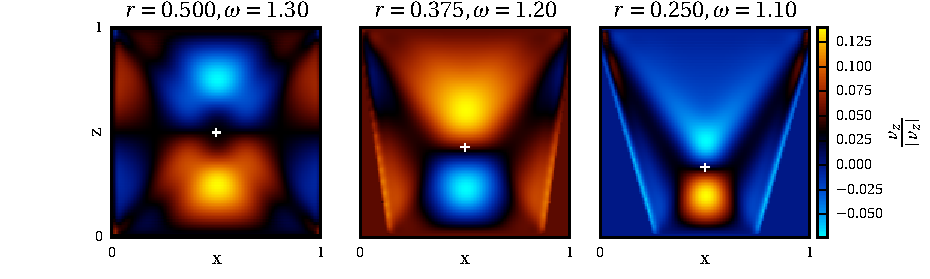
\includegraphics{gfx/cone/transition/phase.pdf}
  \caption{\label{fig:cone:phase}
    Simulation of
  }
\end{figure}

\clearpage

\subsection{Liberating Cone with different Offsets at the Top}

Finally we want to adapt the previous setup which was oriented to





The simulation parameters are given by

\begin{center}
\vspace*{0.7ex}
\begin{tabular}{c|c|c|c|c|c|c|c }
%\begin{tabular}{p{0.1\linewidth}| p{0.1\linewidth}| p{0.1\linewidth}|  p{0.1\linewidth}| p{0.1\linewidth}| p{0.1\linewidth} }
$\leftarrow r \rightarrow$ & $ \leftarrow  \omega \rightarrow $ & $\Delta t$ & $\Delta x$ & $c^2$ & \Ekman  & $l_x, l_y, l_z$ & $T_{end}$\\
\hline
$[0,\; 0.5], \Delta r =0.125$ & $[0.2,\; 2], \Delta w = \nicefrac{1}{10}$ & $10^{-5}$ & $\nicefrac{1}{128}$ & 500 & $10^{-4}$  & (1, 1, 1) & 100\\
\end{tabular}
\vspace*{0.7ex}
\end{center}


\begin{figure}[!pt]
  \centering
  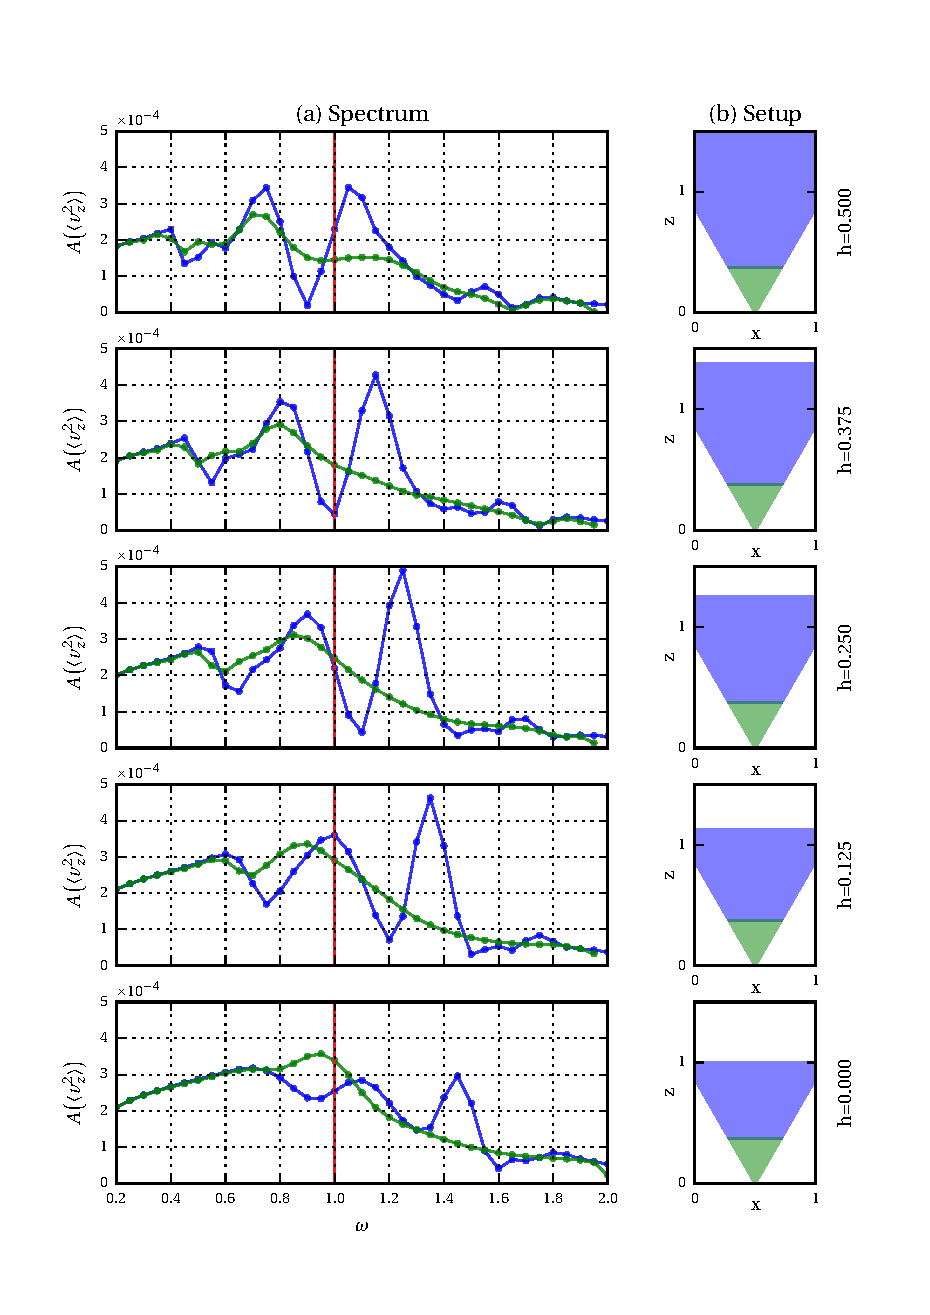
\includegraphics{gfx/cone/final/transition.pdf}
  \caption{\label{fig:cone:finaltransition}
    Simulation of
  }
\end{figure}


2 bilder vgl different alpha

\begin{figure}[!bp]
      \centering
        \resizebox{0.5\textwidth}{!}{
       \import{gfx/cone//}{comparison.pdf_tex}
      }
      \caption{Numerical setup of the cone, oriented on the experiment. The total heigth
         is given by $h$, whereas the height of the cone is set to $h_c$.
      The winkel alpha defines the slope and $h_t$ the cutoff from the bottom.}
      \label{cone:theorie}
\end{figure}
\subsection{Results \& Discussion}

-description\\
-verfahren und serie\\
-diskussion oberer rand\\
-eigenschaften und influence oberer rand \\


Finally
-nun cone mit und ohne spitze
-teste den einfluss der oberen kante blablabla
-serien vergleich diskussion\
-helizität diskussion\\

In order to test
As a first test

\subsection{Discussion}


\section{Summary}
freeslip besser




